

\documentclass[runningheads]{llncs}

\usepackage{graphicx}
\usepackage{xcolor}
\usepackage[hyphens]{url}
% Used for displaying a sample figure. If possible, figure files should
% be included in EPS format.

\begin{document}

\title{Filtering Of Inappropriate Video Content: A Survey}
%\titlerunning{Abbreviated paper title}
% If the paper title is too long for the running head, you can set
% an abbreviated paper title here

\author{
Mahmoud Taha\inst{1}\orcidID{0000-0002-9148-6960}
\and
Ahmed Zakey\inst{1}\orcidID{0000-0002-9148-6960}
\and
Abdulwahab Al-Sammak\inst{1}\orcidID{0000-0002-9148-6960}
} 

\authorrunning{M. Taha \and A. Zakey \and A. Al-Sammak}

\institute{Faculty of Engineering at Shoubra, Cairo, Egypt\\\url{http://feng.bu.edu.eg/feng/en/} }

\maketitle % typeset the header of the contribution

\begin{abstract}
%15--250 words.

With the emergence of screened films, Video content classification has become ubiquitous. Television films and Internet sites films are a big source of violence that may psychologically hurt teenagers. Although recently, Deep learning video classification has been developed quickly, a Comprehensive survey is needed to summarize the previous work done in this field. Therefore, this survey paper shows the common methods used in video classification. We further discuss the importance of filtering sensitive content such as (pornography, violence, gory, etc.) because of the increasing consumption of films by people of all ages. Several real-world verdict cases are similar scenarios to films with many scenes of violence. As deep learning has shown big success in computer vision areas, researchers are giving it a lot of attention.

\keywords{Video filtering \and Video analysis \and Video classification.}

\end{abstract}
\section{Introduction}

 Videos can be categorized into many categories. It is possible to classify them according to the content, such as educational or entertainment content, or to classify them according to the type of images from which these videos were prepared, such as two-dimensional films, three-dimensional films, and cartoon films. As for the video content, there is much content that should be filtered to protect children, including sexual content, violence and the content that causes autism. We will present some previous attempts aimed at filtering some or all of the inappropriate content from some types of videos.\\
 
 Pornography has many common definitions in the psychological and scientific fields. One of the most known definitions states that pornography \cite{mosher1988pornography} is any commercial product in the form of fictional drama designed to elicit or enhance sexual arousal. Another definition states that it is any printed or visual material containing the explicit description or display of sexual organs or activity, intended to stimulate sexual excitement and whatever you choose from the previous definitions, they all agreed that pornography is all about sexual excitement and show the bounds.\\
 
Violence detection is a strenuous problem due to the heterogeneous content and variable quality of videos. Supervised classification is a fundamental task in machine learning. violent scenes are associated with nude colour in video frames and groans and moans in the audio. there are cases like wrestling in which we may have false-negative or false-positive results. Traditional video filtering methods only work on a single dimension of features such as video frames colour analysis or video. When multiple dimensions of features such as ( image frames colours, audio content, motion in the frame sequence of video, or emotions of the audience ) are used, how can these features be integrated to perform accurate classification? The existence of such features raised the need of multi-feature learning \cite{xu2013survey}, \cite{zhao2017multi} \cite{short2012review}. \\

{\ colour {red}For multi-feature classification, it may be required to identify classes of subjects that differ in each of the data views.} In the past two decades, video content filtering has attracted more and more attention, so it is necessary to summarize the state of the art and outline open problems and future enhancements. We divide the video filtering methods into model-based approaches and similarity-based approaches. Generative approaches learn the distribution of the features and use generative models to represent video classification. Discriminative approaches optimize a function that tries to keep down the different classes’ average similarity. Discriminative approaches have many types based on the combination method of the multi-feature information such as common eigenvector matrix or common indicator matrix.\\

we can also divide previous work done into two categories one of them is the targeted content to be filtered such as ( violence only , pornography only or both of them ) , the second category can be the targeted media type such as ( real videos only , animation cartoons only or both of them ), as shown in fig \ref{content_types}. \\
\begin{figure}
\centering
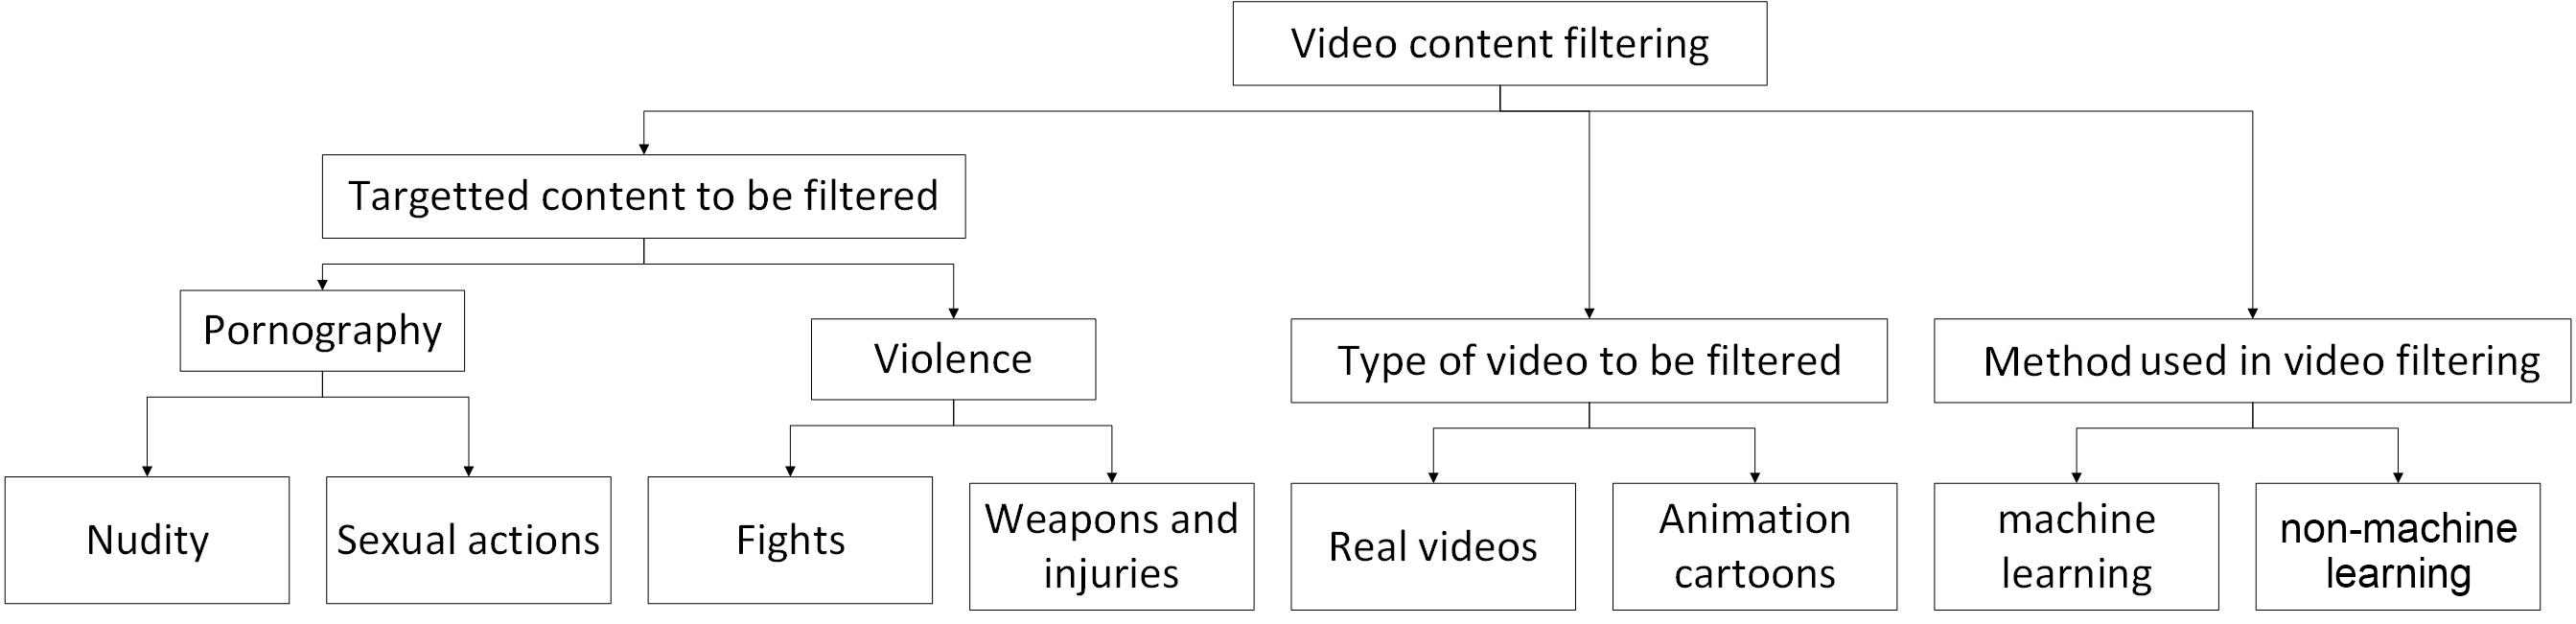
\includegraphics[width=\textwidth]{figures/types_v3.jpg}
\caption{Types of Inappropriate content filtering} \label{content_types}
\end{figure}

As far as what this paper is concerned, The video filtering and video analysis papers of are published in top machine learning venues like the International Conference on Machine Learning (ICML) \cite{srivastava2015unsupervised}, Neural Information Processing Systems (NIPS) \cite{simonyan2014two}, IEEE International Conference on Computer Vision and Pattern Recognition (CVPR) \cite{karpathy2014large}, International Conference on Computer Vision (ICCV) \cite{li2017leveraging}, Association for the Advancement of Artificial Intelligence (AAAI) \cite{sachan2013sports}, International Joint Conference on Artificial Intelligence (IJCAI) \cite{fan2018watching}. \\

Although video filtering has shown considerable success in practice, some open problems limit its advancement. We explain several open problems and hope that readers can have a better version of the automatic video filtering using deep learning. This paper is organized as follows. In section 2, we introduce the existing deep learning methods for video filtering. In section 3, we review video filtering using different approaches other than deep learning. In Section 4, we review previous work done that targets nudity and pornography. Section 5 shows the previous work that targets violence and injuries. In section 6, we introduce some papers that work on animated cartoon classification. Section 7 shows different performance evaluation techniques. In section 8, we introduce a list of data-sets used in video filtering and video content analysis. In Section 9, we show a list of challenges in video filtering research. Finally, we introduce the conclusions.\\

Paper \cite{xu2015discriminative} proposes a discriminative method for event detection using video representation. The focus is to leverage Convolutional Neural Networks (CNNs) to improve event detection.it begins by the frame-level extracting by CNN descriptors then it generates video level representations.\\

\section{Video filtering using machine learning approaches}

Among all media types (e.g., texts and audio ), images are the most used pornography carrier. Since pornography often has skin exposure, skin detection is commonly used for pornography detection. However, because skin detection is challenging, the Approaches used have a limited generalization ability. Vu Lam and Duy-Dinh Le introduced MediaEval \cite{demarty2013mediaeval} that combined the trajectory-based motion features with SIFT-based and audio features. their results show that the trajectory-based motion features still have very competitive performance. the combination with image features and audio features can improve overall performance for violence detection in videos.\\

paper \cite{wang2013action} states that recently dense trajectories were shown to be an efficient video representation for action recognition and achieved state-of-the-art results on a variety of data-sets. they improve performance by taking into account camera motion to correct them. To estimate camera motion, matching feature points between frames using SURF descriptors and dense optical flow is important.\\

Human motion is in general different from camera motion and generates inconsistent matches. To improve the estimation, a human detector is employed to remove these matches. Given the estimated camera motion, paper \cite{wang2013action} removes trajectories consistent with it and uses this estimation to cancel out camera motion from the optical flow. This significantly improves motion-based descriptors, such as HOF and MBH. Focusing on filtering real-time videos, Nevenka and Radu produced an effective patent \cite{dimitrova2015system} that automatically filters multimedia program content in real-time based on stock and user-specified criteria. It includes one or more multimedia processors, which analyze incoming visual, audio, and textual, content and compares the resultant analysis to specific user-specified or selected criteria.\\

In paper \cite{tofa2017inappropriate}, nude detection is implemented with the use of two algorithms. The first algorithm detects humans from the processed frames and then crop them out. Then the second algorithm is the nude detection algorithm used to determine if the images are nudes or not. the technique used in this paper has many problems. first is that	while detecting nudity, it fails to properly classify black and white images as containing nudity or not because this paper is based mainly on skin colour. When a person is wearing a skin-toned dress the paper's algorithm gives a false positive result and it also fails to detect nudity if most of the body portion is not included in the video frames. paper \cite{qi2000integrating} presents a system developed for content-based news video browsing for home users. This system integrates the audio-visual as well as text detection and NLP technique analysis to extract structure and content information of news video and to organize and categorize news stories.\\

Jin \cite{jin2018pornographic} used weighted multiple instances learning to model each image as a bag of regions and train a generic region-based recognition model taking into account the degree of pornography for each region. He shows that the key pornographic contents often are located in local regions in an image, and the background regions may be destructive. He stated that there are two main pornographic contents: the private body parts, and sexual behaviours. We perform bounding box annotation for these key pornographic contents in the training set, and for the sexual behaviour, Using annotations, there are only a small number of annotations (less than 10) required for both types of pornographic contents. each image X is modeled as a bag of
n regions $ { x_{i}|i = 1, ... , n } $ . Given a region, the deep CNN extracts layer-wise representations from the first convolutional layer to the last fully connected layer. His CNN architecture is inspired by the GoogLeNet model \cite{szegedy2015going}. The final results for this method are shown in fig \ref{roc_map}. \\

\begin{figure}
\centering
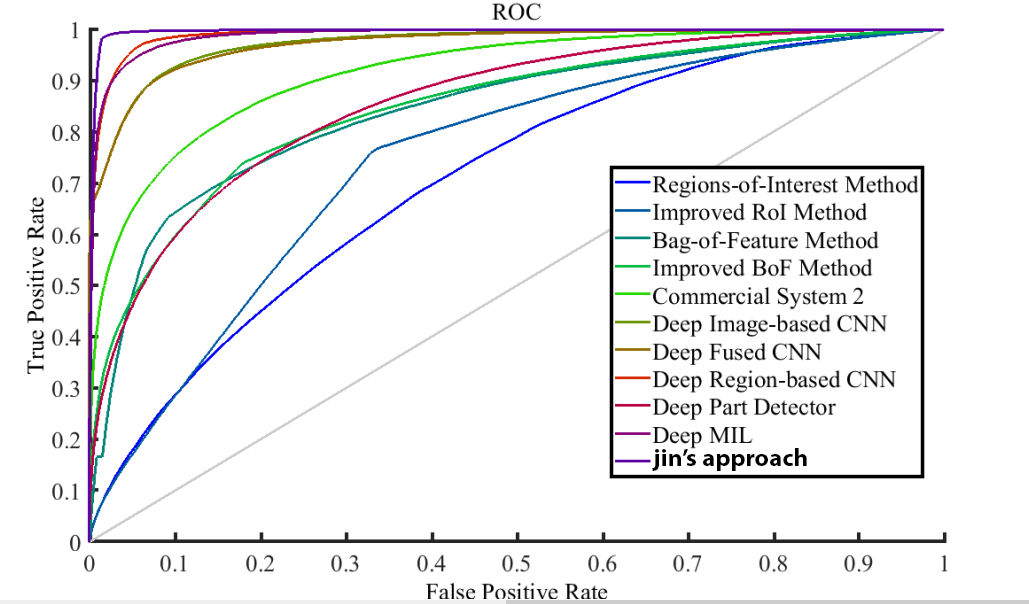
\includegraphics[width=.7\textwidth]{figures/roc.PNG}
\caption{ROC curve of different methods for pornographic image recognition.Jin's method significantly outperforms traditional methods.In particular,He achieve accuracy of 97.52\% TPR at 1\% FPR } \label{roc_map}
\end{figure}

\section{Video filtering based on non-machine learning approaches}
Due to some obstacles in machine learning such as data acquisition and powerful resources required for training, Some researchers tried to avoid using machine learning and use fixed algorithms instead.\\

\subsection{Blocking Adult Images Based on Statistical Skin Detection \cite{zheng2004blocking} }

One of the most important papers worked in images filtering without using machine learning directly to train on images is this paper \cite{zheng2004blocking}. Paper \cite{zheng2004blocking} shows a method to filter adult images using statistical algorithms. Human skin pixels detection from an image is performed. MaxEnt method used for inferring models from a data set. It works as follows: (1) choose relevant features (2) compute their histograms on the training set (3) write down the maximum entropy model within the ones that have the feature histograms as observed on the training set (4)
estimate the parameters of the model (5) use the model for classification. The output of skin detection is a map indicating the probabilities of skin on pixels shown in fig [ \ref{skin_map} ]. After that paper \cite{zheng2004blocking} computes a sequence of 9 features from this skin
map which form a feature vector and uses the fit ellipses to catch the characteristics of skin distribution. Two
ellipses are used for each skin map—the Global Fit Ellipse (GFE) and the Local Fit Ellipse (LFE). A multi-layer perceptron classifier is trained for these features. It is a semi-linear feed-forward net with back-propagation
of error. Skin detection is never perfect and analysis of text in images may increase the accuracy of classification.\\

\begin{figure}
\centering
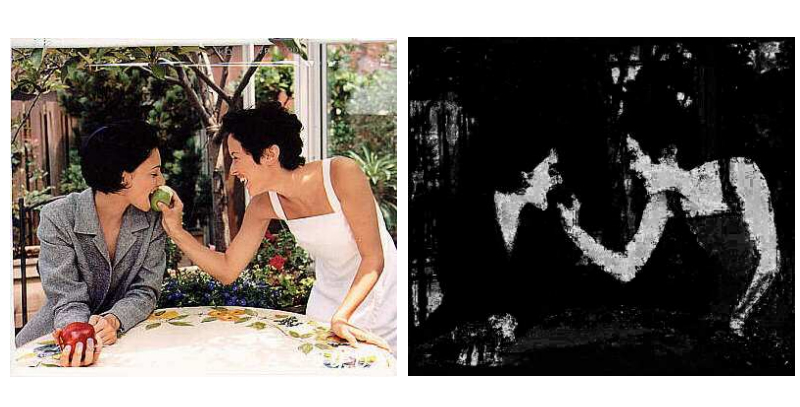
\includegraphics[width=1\textwidth]{figures/skin_map.jpg}
\caption{On the right: original color image. On the left: the corresponding skin map output by TFOMure. } \label{skin_map}
\end{figure}

\section{Video Filtering Targeting Pornography}
Due to research report \cite{quadara2017effects}, The term pornography can be defined as any sexually explicit material that is generally intended to sexually arouse the audience. In this section, we show different papers and researches that target filtering pornography in videos regardless of the used technique for filtering or the type of targeted videos.\\

paper \cite{perez2017video} shows that motion information in videos can help to classify difficult cases of pornography. Only a few works have used motion information in automatic video filtering such as Space-Time Interest Points (STIP)\cite{laptev2005space} and Temporal Robust Features (TRoF) \cite{moreira2016pornography}. As shown, Some researches sought to extract motion information by feeding frames to the CNNs \cite{le2011learning}, while others opted for feeding this information to the network through a previously computed Optical Flow Displacement Fields image representation \cite{simonyan2014two}.\\

In paper \cite{perez2017video}, Authors reported a Summary of approaches on skin, nudity or pornography detection. A good survey on this point can be found in this paper.\\

\section{Video Filtering Targeting Violence}
In psychology, violent scenes are defined as scenes one would not let an 8-year-old child see because they contain physical violence. This is the subjective definition. The objective definition is physical violence or accident resulting in human injury or pain. In this section, we show different papers and researches that target filtering violence, injuries and fights in videos regardless of the used technique for filtering or the type of targeted videos.\\

Violence classification started by detecting blood and screams using sound features \cite{giannakopoulos2006violence}. In paper \cite{das2019violence}, A system that identifies violence in each frame by extracting HOG features and classifies it using a random forest classifier.
this system shows low accuracy even it didn't require a GPU for computations.
Recent researches like  \cite{simonyan2014two} and \cite{sakthivinayagam2019violence} detect violence and fight using deep learning architectures such as long short-term memory (LSTMs), and two-stream CNN's \cite{simonyan2014two} and convolutional neural networks (CNNs) in \cite{sakthivinayagam2019violence}. These methods show better accuracy than previous algorithms used.\\

Author in paper \cite{abdali2019robust} used a pre-trained CNN architecture VGG-19 \cite{simonyan2014very} followed by LSTM. The results from CNN of each frame are grouped and fed to the LSTM. this model has an accuracy of 94.765\% which is a good performance.  Qichao Xu \cite{xu2019localization} used the FlowNet 2.0 \cite{ilg2017flownet} model for estimating optical flow and the pre-trained SSD-VGG16 for human detection. The localization phase is combined for predictions after a two-stream C3D network \cite{tran2015learning} is trained on the active regions. The methodology from \cite{song2019novel} detects violence using keyframe extraction algorithm and 3D ConvNet achieving 93.5\% accuracy with the Crowd violence dataset. Keçeli at al. \cite{kecceli2017violent} used AlexNet with transfer learning and utilized the Lucas-Kanade method for finding the optical flows of frames. Templates are made from the optical flow and fed as input to AlexNet for feature extraction. After using multiple classifiers, The best results have been obtained from the SVM classifier. In paper \cite{sharma2021fully}, Auther used an LSTM network to perform sequence prediction on the vectors resulting from a convolution neural network that extracts the spatial feature as shown in fig[\ref{violenceSharmaCnn}]. For the spatial feature extraction, The architecture of Xception \cite{chollet2017xception} network has been used with the pre-trained model on the ImageNet dataset \cite{krizhevsky2012imagenet}.

\begin{figure}
\centering
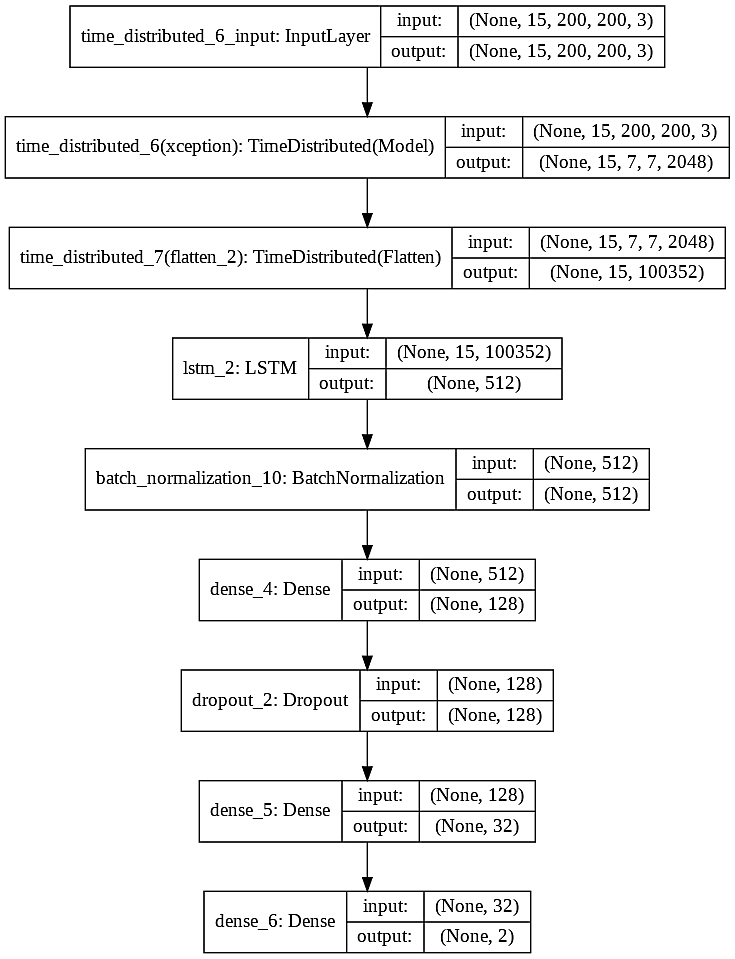
\includegraphics[width=0.6\textwidth]{figures/violenceSharmaCnn.png}
\caption{Model Architecture for Sarthak Sharma Paper.} \label{violenceSharmaCnn}
\end{figure}

for paper \cite{halder2020cnn}, they predict sequences in consecutive frames using both spatial features and temporal or time-related features as well. The Convolutional Neural Network (CNN) used in this paper, is composed of an input convolutional layer followed by three layers of convolution and max pooling. The kernel size for each convolutional layer is 3 × 3. 64 kernels are used in each convolutional layer. The output from each convolutional layer after passing through “relu” activation as shown in fig[\ref{violenceHalderCnn}].\\

\begin{figure}
\centering
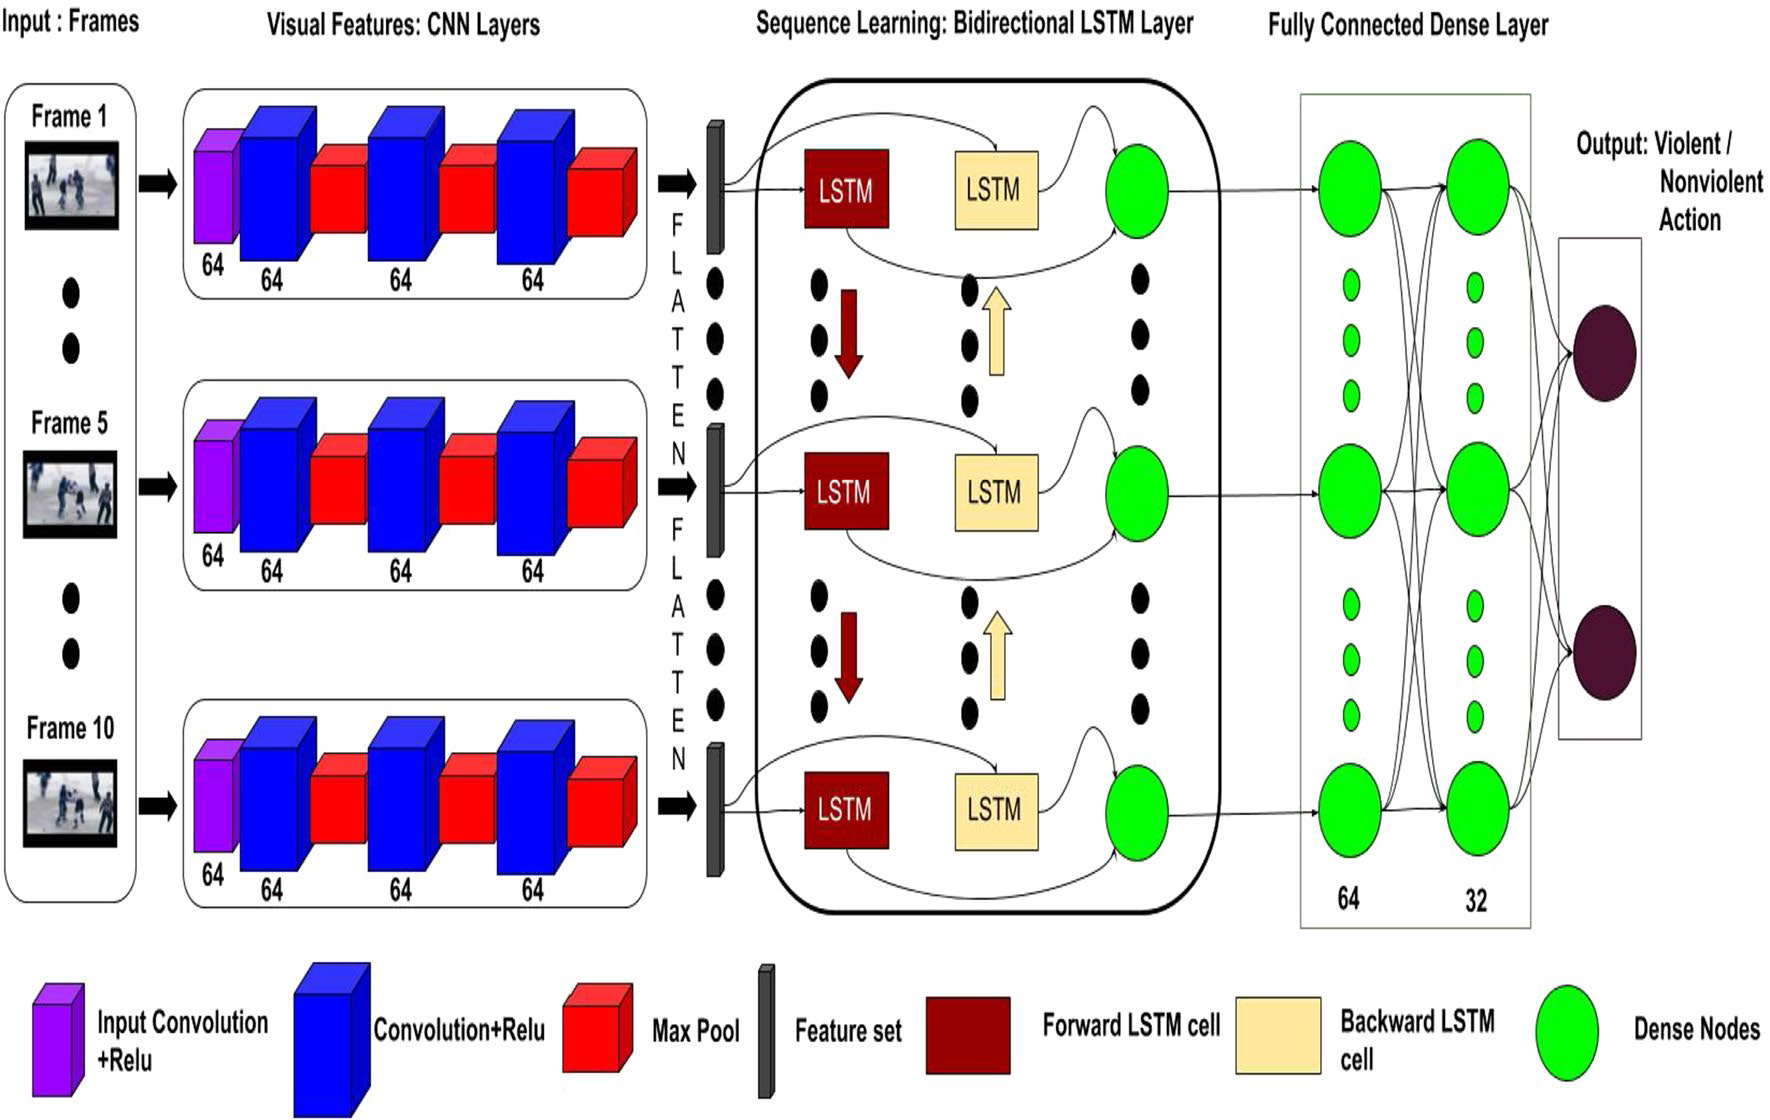
\includegraphics[width=0.9\textwidth]{figures/violenceHalderCnn.png}
\caption{Model Architecture for Rohit Halder Paper.} \label{violenceHalderCnn}
\end{figure}

As soon as the blood is visually present in the image, Additional tags are required to represent the proportion of it in the image. These tags can be: unnoticeable, low, medium, high with the following meanings:
\begin{itemize}
 \item unnoticeable: there are some blood pixels no more than 5\% of the image
 \item low: pixels represent blood are is in [ 5\% and 25\% ].
 \item medium: pixels represent blood are in [ 25\%, 50\% ].
 \item high: pixels represent blood are higher than half pixels of the image.
\end{itemize}

Fights can be annotated in different tags:
\begin{itemize}
 \item 1 vs 1: fighting between only two people.
 \item small: for a group of people less than 10 persons.
 \item large: for a large group of people greater than 10 persons.
 \item distant attack: somebody is shot.
 \item Human against animal fights.
 \item Explosions, Scream and gunshot sounds can facilitate correct classification.
\end{itemize}

\section{Filtering Animated Cartoons}

Child pornography \cite{tate1990child} is an important problem in cyber-security. The increased use of the internet increased the circulation of offensive images of children.

\subsection{Unsupervised Discovery Character Dictionaries in Animation Moves \cite{somandepalli2018unsupervised}}

This paper \cite{somandepalli2018unsupervised} shows a method to create a characters' dictionary for an animation video using unsupervised learning. A set of eight movies was used to evaluate the method suggested in the paper and can be used for labelling animation characters. Character dictionaries in animated cartoons can be the first step for cartoon content analysis. Paper \cite{somandepalli2018unsupervised} uses a deep neural network natural objects detector to identify some initial characters. These initial characters are pruned using visual object tracking. A character dictionary is then generated for each movie.\\

One of the best results for the method mentioned is a generalization for animation movies \cite{zheng2004blocking} at scale. AS shown in fig[\ref{cartoon_chars}], there is a high degree of heterogeneity of animated cartoon characters, So Paper \cite{somandepalli2018unsupervised} can identify both 2-dimensional and 3-dimensional characters with a different collection of character designs, But In digital animations, objects can be fictional so object detection can be more challenging. paper \cite{somandepalli2018unsupervised} uses a deep neural network called Multi-Box \cite{erhan2014scalable} , \cite{szegedy2014scalable} designed for object detection. Multi-Box was used only to generate a set of character candidates. The performance is quantified by comparing the reference characters with the output dictionaries from the method used.\\

Due to the success of AlexNet, deep learning has become the most common method for image recognition. A few years ago, R-CNNs were developed to deal with the object detection task but three were many problems with the above networks such as too-long data training and multiple phases training. As a result of these problems, new networks were developed such as YOLO (You Only Look Once) and SSD MultiBox (Single Shot Detector). SSD MultiBox was released in 2016 and reached new records for object detection tasks, scoring over 74\% mAP (mean Average Precision) at 59 frames per second on standard datasets such as COCO.\\

\begin{figure}
\centering
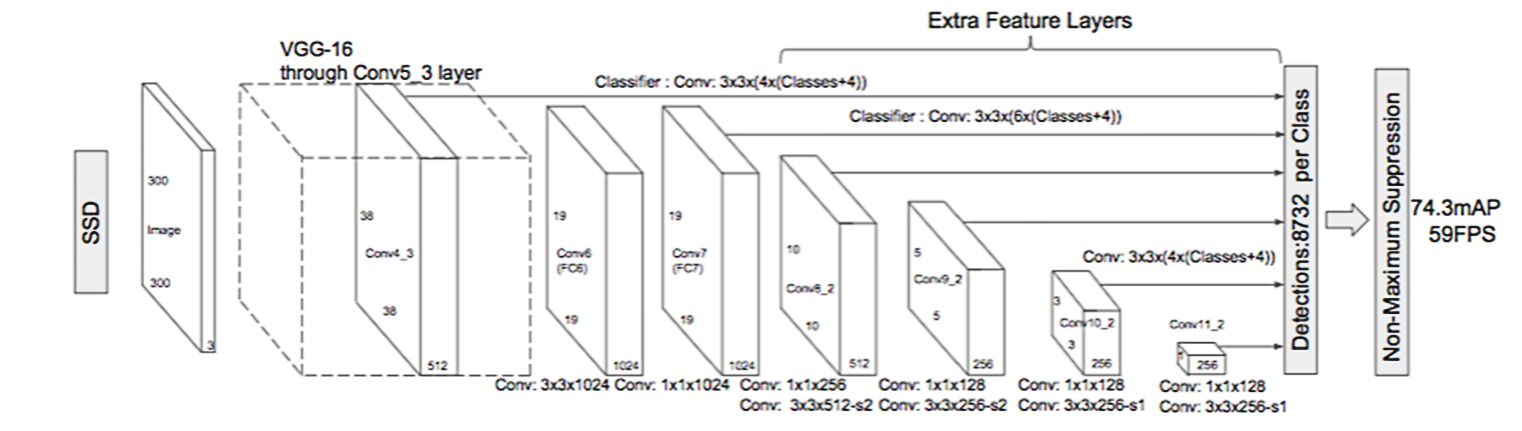
\includegraphics[width=1\textwidth]{figures/multibox.png}
\caption{SSD MultiBox network architecture. } \label{ssd_multi_box}
\end{figure}

As shown in the fig [ \ref{ssd_multi_box}, \ref{multi_box_arch2} ], It’s called Single Shot because object localization and classification are achieved in a single forward pass of the network built on the venerable VGG-16 architecture with 1x1 convolutions that helps in dimension reduction but discards the fully connected layers. MultiBox’s loss function also combined two components confidence loss which uses categorical cross-entropy and location Loss which uses L2-Norm. The expression for Loss can be stated as $ multibox_loss = confidence_loss + alpha * location_loss $.\\

\begin{figure}
\centering
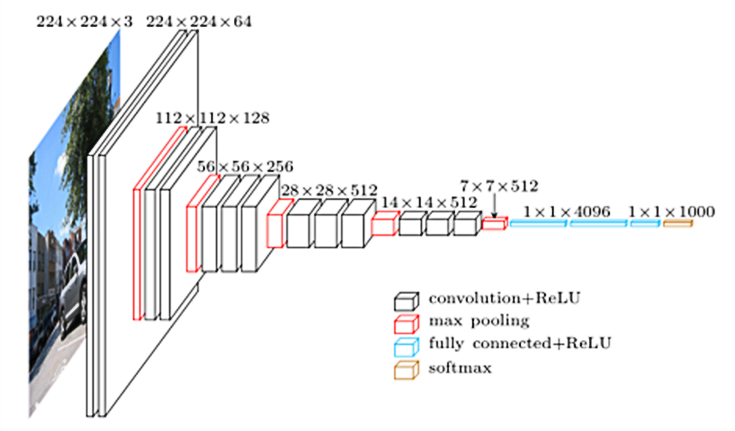
\includegraphics[width=1\textwidth]{figures/multi_box_arch2.png}
\caption{MultiBox network architecture.}
\label{multi_box_arch2}
\end{figure}

In MultiBox, the researchers created what we call priors, which are pre-computed, fixed-size bounding boxes that closely match the distribution of the original ground truth boxes. In fact, those priors are selected so that their Intersection is greater than 0.5. It is a better strategy than starting the predictions with random coordinates. The resulting architecture contains 11 priors per feature map cell (8x8, 6x6, 4x4, 3x3, 2x2) and only one on the 1x1 feature map, resulting in a total of 1420 priors per image. Assuming we have configured 2 diagonally opposed points (x1, y1) and (x2, y2) for each b default bounding boxes per feature map cell, and c classes to classify, on a given feature map of size $ f = m * n $, SSD would compute $ f * b * (4 + c) $ values for this feature map. Non-maximum suppression: boxes with a confidence loss threshold less than (e.g. 0.01) and IoU less than (e.g. 0.45) are discarded, and only the top N predictions are kept.\\

\begin{figure}
\centering
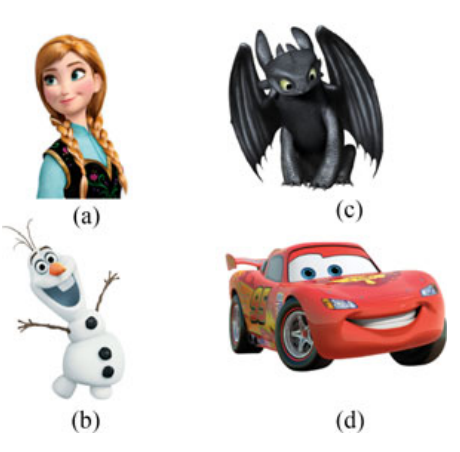
\includegraphics[width=.4\textwidth]{figures/cartoon_chars.png}
\caption{Examples of the heterogeneity of animated cartoon characters. } \label{cartoon_chars}
\end{figure}

\subsubsection{Future work}
 One of the drawbacks of paper \cite{somandepalli2018unsupervised} is using an object detector that was trained with natural human images. As a result, the Authors plan to solve this issue using transfer learning. Authors also suggest using the relevant exemplars and associated cluster as a single unit to facilitate animation video classification.\\

\subsection{Video Analysis for Cartoon-like Special Effects}

Paper \cite{collomosse2003video} demonstrates a system for rendering motion within any artistic video. Key to paper \cite{collomosse2003video} work is the analysis of trajectories. it uses additional ‘ghosting’ lines which indicate the trailing edge of the object as it moves along the streak lines, like in fig [\ref{cues}]. Ghosting lines are usually perpendicular to streak lines. Deformation is often used to emphasize motion, and a popular technique is a squash and stretch in which a body is stretched tangential to its trajectory. they use a robust motion estimation technique in paper \cite{torr1995motion} for camera motion and use paper \cite{harris1988stephens} for Harris interest points detection in video frames. they calculate contour motion by a linear conformal affine transform (LCAT) in the image plane. Like camera motion correction, interest points \cite{harris1988stephens} are identified within the tracked object. there are many cases in which point correspondences can not be found such as small feature areas. As a result, coloured markers may be attached to the subject and later be removed automatically. they use tracked features mutual occlusion over time to determine partial depth ordering.\\

As mentioned in paper \cite{harris1988stephens}, The trajectory of any object can be defined by its centroid trajectory. Due to a fixed common basis for each frame, paper can estimate the velocity and acceleration of the centroid of the object. At each instant, they build a curvilinear basis frame using the centroid trajectory.As a result, paper can calculate the point in the world frame with equation $x_t(r,s) = \mu (r) + sn(r)$. but this equation fails on collision points. they have a buffer for saving pixels that occlude the tracked object. occlusion pixels are one that has the Euclidean distance between predicted colour and observed colour and exceeds a threshold.\\

\begin{figure}
\centering
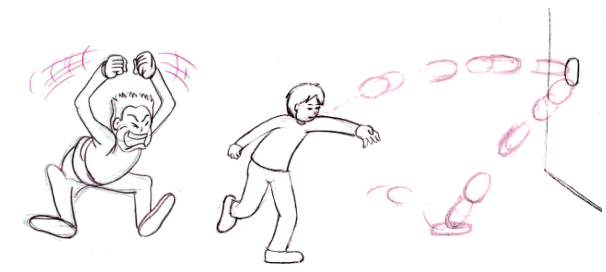
\includegraphics[width=.5\textwidth]{figures/cues.png}
\caption{Examples of cues used in animation videos} \label{cues}
\end{figure}

An animated object can be defined as a distorted version of the original. it is needed to bend an object along the arc of its centroid as we may get unattractive results if we use only squash and stretch tangential to instantaneous motion. The robustness of the algorithm could be evaluated both with ground truth comparisons for measures such as velocity, as well as processing sequences exhibiting distinctly non-planar motion.\\

\subsubsection{Future work}
paper \cite{collomosse2003video} suggests many aspects that may be improved such as improving occlusion handling. they believe the future work will examine alternatives for Spatio-temporal video analysis.\\

\section{Performance evaluation}
Recent efforts show that combining multiple features, such as static appearance, motion features and acoustic features, can perform event detection.for the case \cite{perez2017video}, the target was to implement the model in a mobile device with limited resources. In this regard, GoogLeNet is superior to VGG as the former has a learned model with only 40 MBs against a learned model of 533 MBs of VGG.in table  [\ref{tab_results}], we show several approaches with the reported results from other methods using the Pornography-800 dataset.Also In figure \ref{fig_results}, we show results for paper \cite{jin2018pornographic} compared to many different methods. \\

\begin{table}
\caption{Results on the Pornography-800 dataset reported with the average performance and standard deviations using the dataset's 5-fold evaluation protocol.}
\label{tab_results}
\begin{tabular}{|p{5cm}|p{4cm}|p{3cm}|}
\hline
Method & Solution & Accuracy \\
\hline
CNN & Moustafa\cite{moustafa2015applying} & $94.1 \pm 2.0$ \\
\hline
CNN & Mid-level fusion (OF) & $97.9 \pm 0.7$ \\
\hline
CNN & Late fusion (OF) & $97.9 \pm 1.5$ \\
\hline
CNN & Static - Fine-tuned & $97.0 \pm 2.0$  \\
\hline
CNN & Motion - Optical flow & $95.8 \pm 2.0 $ \\
\hline
BoVW-based & Moreira et al.\cite{moreira2016pornography} & $95.0 \pm 1.3$ \\
\hline
BoVW-based & Caetano et al.\cite{caetano2016mid} & $92.4 \pm 2.0$ \\
\hline
BoVW-based & Valle et al.\cite{valle2011content} & $91.9 \pm NA$ \\
\hline

\end{tabular}
\end{table}


\begin{figure}
\centering
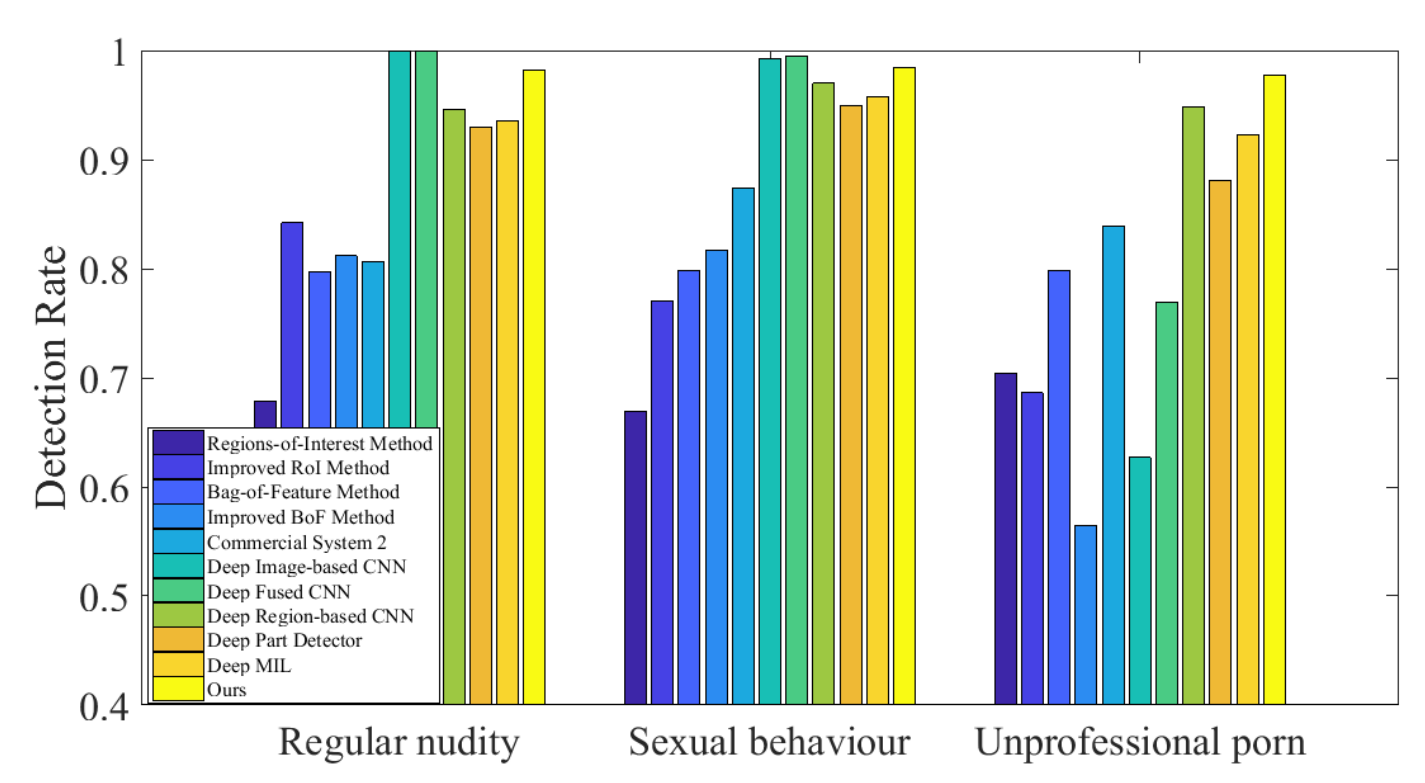
\includegraphics[width=.8\textwidth]{figures/results.png}
\caption{Comparing results for paper \cite{jin2018pornographic}  with other different methods.} \label{fig_results}
\end{figure}

\section{List of data-sets}
One important obstacle in this research is the dataset used for DNN learning. Almost all available datasets in the scientific field are for real human videos so it may be needed to search for a good animated cartoons dataset.See table [\ref{tab_dataset}].

\begin{table}
\caption{List of data-sets used in Inappropriate content analysis}
\label{tab_dataset}
\begin{tabular}{|p{3cm}|p{1.5cm}|p{7.5cm}|}
\hline
Name & Datatype & Description \\
\hline
\hspace{0pt}Danbooru2018 \cite{Danbooru2018} & images & A 300 GB Crowd sourced and Tagged 3.33m+ anime images illustration dataset classified into 3 categories: safe, questionable and explicit (pornographic). \\
\hline
Safebooru \cite{Safebooru} & images & A 250 MB Crowd sourced and Tagged 2.4m+ anime images with tagged description. \\
\hline
Tagged Anime Illustration \cite{TaggedAnimeIllustration} & images & A 36 GB Crowd sourced and Tagged anime images with SFW or pornography tagged description. \\
\hline
youtube8m \cite{youtube8m} & videos & A big dataset of various types and activities tagged from YouTube. \\
\hline
UCF-101 \cite{UCF-101} & videos & A big dataset of various types of human action recognition videos.\\
\hline
kinetics \cite{kinetics} & videos & A dataset of various types of all human action recognition videos. \\
\hline
VSD2014 \cite{VSD2014} & videos & A dataset of violent videos or most popular Hollywood films. \\
\hline
Pornography-800 (NPDI-DCC-UFMG) \cite{Pornography-800} & videos & A dataset of 80 hour videos of 400 pornographic and 400 non-pornographic videos. \\
\hline
Sexualitics \cite{Sexualitics}& metadata & A dataset of metadata of all video on two big pornographic westies XHamster and Xnxx. \\
\hline

\end{tabular}
\end{table}


\section{Challenges}
There are still a lot of challenges in video filtering fields due to the huge variety of types of videos. As an example, one important question to answer is what exactly will we detect in videos, we have a lot of choices ( Guns, weapons and alcohols or Blood and injuries or Nudity or Shouting and fighting action recognition or Sex action recognition ) or simply detecting all of this. Also, For there are also sub-categories like ( Suggestive sex or Explicit Sex or Paedophilia sex ). as shown in fig[\ref{fig1}], there are different types of cartoon videos and animated graphs like 2-dimensional videos, 3-dimensional videos, stop motion and line drawing. targeted audience age is one of the most important parameters of the filtering process because filtering video for 3-years-old children is different from it for an 18-years-old man watching the same video. the younger the person watching filtered videos, the more content to be filtered in videos.\\\\ This research will target 2-Dimensional as it is most popular in the animated video industry and still needs a lot of research. Also, we will target children as an audience in our filtering as this is still a challenging problem in video filtering. Watching porn films wrongly for children can cause a delay in the child's developmental stages, and it can also cause anaphylaxis and autism, and give the child a wrong idea about human relationships, and children may commit crimes. Therefore, video filtering for children and cartoon was of special importance to protect society from the risks that may result from this phenomenon.\\
Another question to answer is what is the main data needed to be classified to give us the right classification of the video. The answer to the previous question can be one or multiple of this data type ( frame images of the video, motion sequence between the image frames, voice emotion, Impression of audience and NLP of the speech in the video ), whether you choose one or more of the previous categories but this will affect your accuracy and required work and data-set to accomplish classification task. There are many categories of videos that can be classified working on all of them will need more generalized and trained DNN and more generalized data-set. Videos can be real films or animated cartoons and also can be targeting adults or children. Even Cartoon has many sub-categories like 2-dimensional cartoons, 3-dimensional cartoons and stop-motion cartoons.\\

\begin{figure}
\ centring
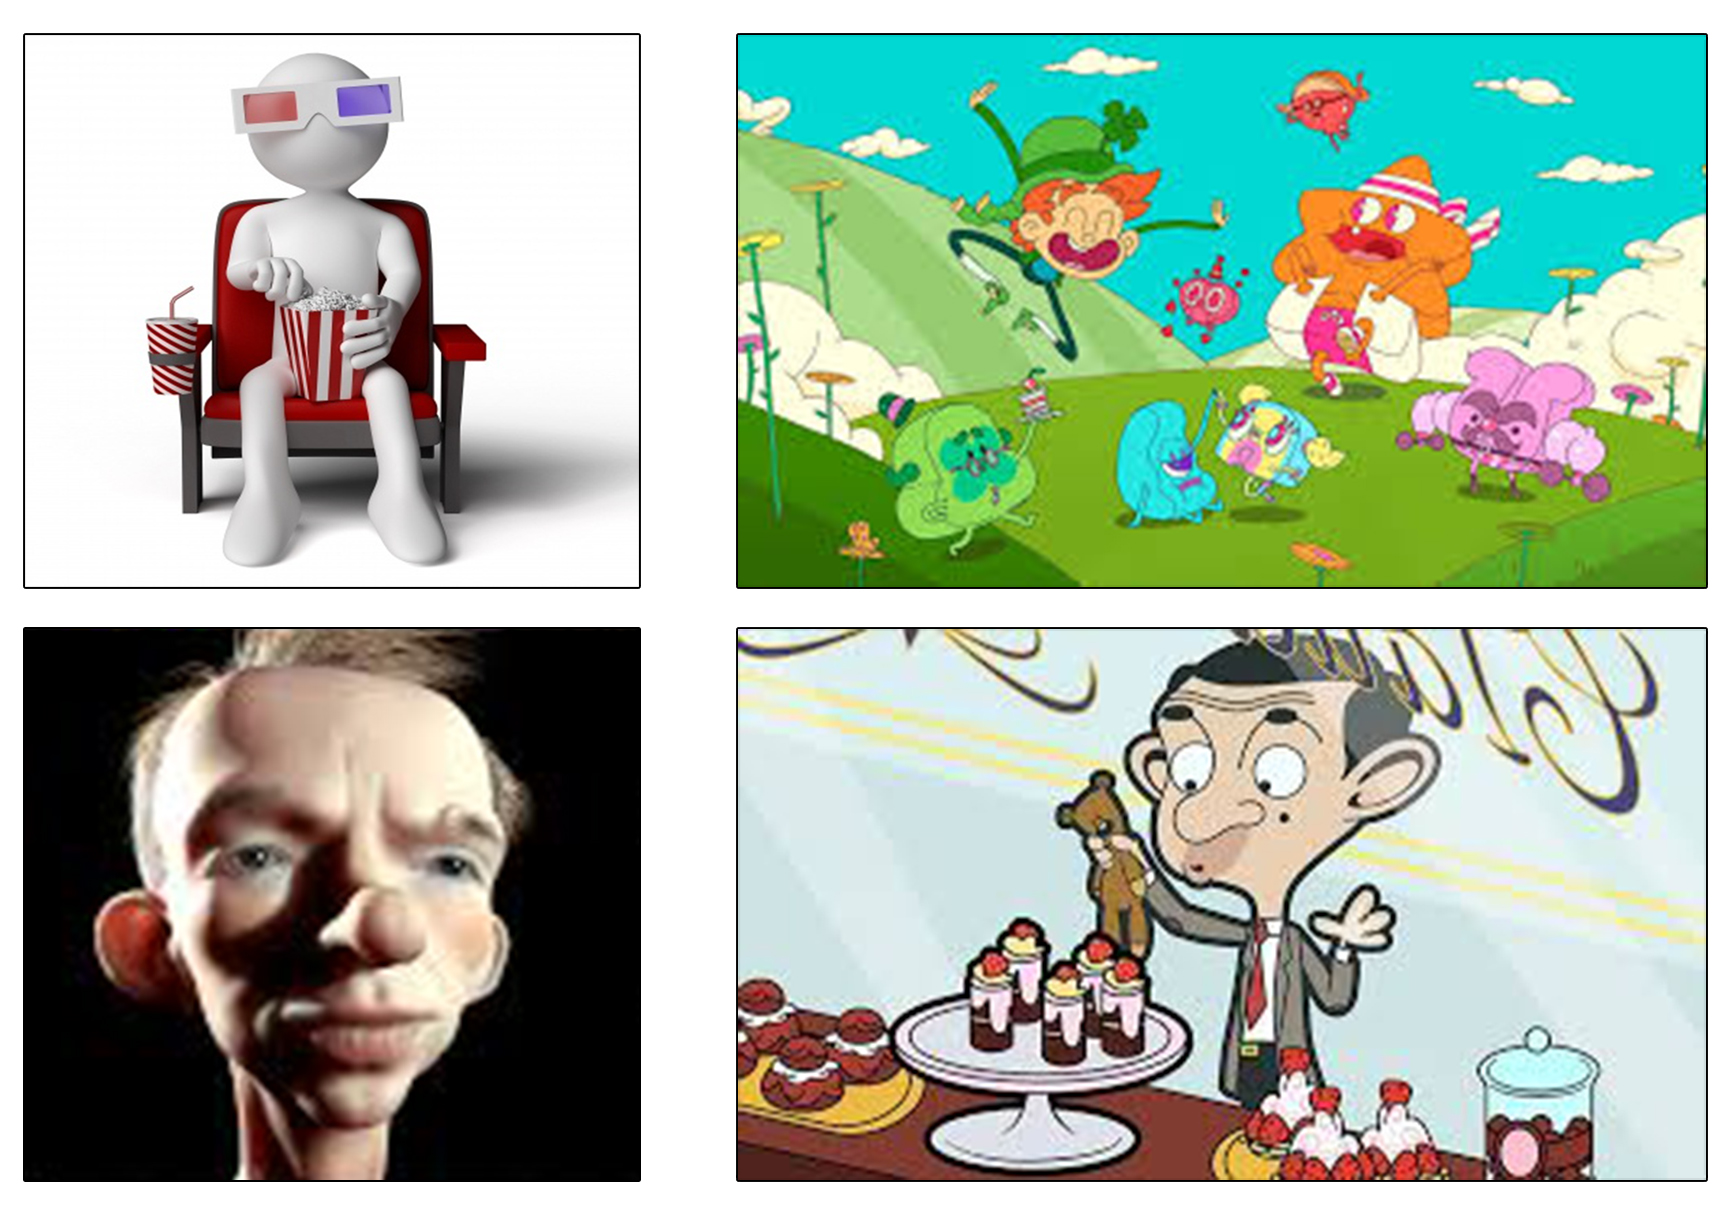
\includegraphics[width=.6\textwidth]{figures/cartoons.jpg}
\caption{Different types of cartoon Animated images.} \label{fig1}
\end{figure}

\section{Conclusion}
The association of Deep Learning with the combined use of static and motion information considerably improves pornography detection. Not only over the current scientific state of the art but also over off-the The Deep Learning solution using only static information is already competitive with state-of-the-art action recognition features.\\

\section{Acknowledgment}
This research is under the supervision of Dr Ahmed Bayiomy Zaki. We thank our colleagues from Shoubra faculty of engineering - Benha university who provided insight and expertise that greatly assisted the research, they may not agree with all of the interpretations/conclusions of this paper.\\

%Sets the bibliography style to UNSRT and imports the 
%bibliography file "ref.bib".
\bibliographystyle{unsrt}
\bibliography{ref}

\end{document}
